\documentclass[10pt,twocolumn]{article}

%% ── Packages ──────────────────────────────────────────────────────────
\usepackage{amsmath,amssymb,amsthm}
\usepackage{mathtools}
\usepackage{microtype}
\usepackage{geometry}
\usepackage{hyperref}
\usepackage{natbib}
\usepackage{tikz}
\usetikzlibrary{arrows.meta,positioning,shapes.geometric,
                circuits.logic.US,fit,calc,patterns,decorations.markings}
\usepackage{pgfplots}
\pgfplotsset{compat=1.18}
\usepackage{booktabs}
\usepackage{array}
\usepackage{caption}
\usepackage{subcaption}
\usepackage{siunitx}
\usepackage{titlesec}
\usepackage{abstract}
\usepackage{enumitem}
\usepackage{bm}
\usepackage{xcolor}
\usepackage{float}

\geometry{
  paperwidth=8.5in, paperheight=11in,
  top=0.85in, bottom=0.9in,
  left=0.65in, right=0.65in,
  columnsep=0.22in
}

\hypersetup{colorlinks=true,linkcolor=black,citecolor=black,urlcolor=black}

\titleformat{\section}{\normalsize\bfseries}{\thesection.}{0.5em}{}
\titleformat{\subsection}{\small\bfseries}{\thesubsection.}{0.5em}{}
\titleformat{\subsubsection}{\small\itshape}{\thesubsubsection.}{0.4em}{}
\titlespacing{\section}{0pt}{6pt plus 2pt}{3pt plus 1pt}
\titlespacing{\subsection}{0pt}{4pt plus 1pt}{2pt}

\renewcommand{\abstractnamefont}{\small\bfseries}
\renewcommand{\abstracttextfont}{\small}
\setlength{\absleftindent}{0pt}
\setlength{\absrightindent}{0pt}

\theoremstyle{plain}
\newtheorem{theorem}{Theorem}
\newtheorem{proposition}{Proposition}
\newtheorem{lemma}{Lemma}
\newtheorem{corollary}{Corollary}
\theoremstyle{definition}
\newtheorem{definition}{Definition}
\theoremstyle{remark}
\newtheorem{remark}{Remark}

\captionsetup{font=small,labelfont=bf,skip=4pt}

%% ── Shorthands ────────────────────────────────────────────────────────
\newcommand{\simA}{\sim_{\!A}}
\newcommand{\DA}{D_{A}(\bm{\varphi})}
\newcommand{\RHP}{\mathcal{R}_{H}^{\Pi}}
\newcommand{\calX}{\mathcal{X}}
\newcommand{\calM}{\mathcal{M}}
\newcommand{\bvphi}{\bm{\varphi}}
\newcommand{\R}{\mathbb{R}}
\newcommand{\E}{\mathbb{E}}

\setlength{\parskip}{2pt}
\setlength{\abovedisplayskip}{4pt}
\setlength{\belowdisplayskip}{4pt}

% ══════════════════════════════════════════════════════════════════════
\title{\textbf{Admissibility Distortion in Latent State Encoders:
A Reachability-Geometric Framework for Fault-Critical
Mechatronic Systems}}

\author{Flyxion\\
  {\small Independent Researcher}}
\date{June 2026}

% ══════════════════════════════════════════════════════════════════════
\begin{document}
\maketitle
\thispagestyle{plain}

\begin{abstract}
\noindent
State encoders embedded in model-based controllers for mechatronic systems
are conventionally evaluated by predictive fidelity metrics---reconstruction
error, prediction horizon accuracy, or spectral coherence between encoder
output and measured plant response. We demonstrate that these metrics are
insufficient for fault-critical planning and control: a formally stated
\emph{Observational--Interventional Separation Theorem} establishes that
encoder observational equivalence does not imply interventional equivalence,
and identifies this as a structural property of the encoder's induced quotient
map rather than an empirical deficiency correctable by additional training data.
The quantity that predictive metrics fail to bound is \emph{admissibility
distortion} $\DA$, defined as the expected Hausdorff distance between
reachability sets of encoder-collapsed state pairs. We derive its decomposition
into collapse-rate and per-collapse severity factors, prove strict monotonicity
under compression, and establish a Bayes-risk floor on any downstream fault
classifier operating on an inadmissible encoder output. Trajectory-rollout
auditing procedures analogous to hardware-in-the-loop (HIL) fault injection
are derived as one-sided witnesses for $\DA > 0$. Applications to brushless
DC motor drive fault isolation, structural health monitoring (SHM) with
piezoelectric sensor arrays, and inverter-fed induction motor flux observers
are developed. The framework subsumes bisimulation-based abstractions and
provides a computable lower bound via bisimulation distortion metrics already
in use for model-based RL controllers.
\end{abstract}

\noindent\textbf{Index Terms:} admissibility distortion, reachability analysis,
state encoder, fault isolation, mechatronics, brushless DC motor, structural
health monitoring, flux observer, model-based control, HIL auditing.

% ══════════════════════════════════════════════════════════════════════
\section{Introduction}

Modern mechatronic systems rely on latent-state encoders---neural networks,
Kalman filter banks, principal-component projections, or learned embedding
networks---to compress high-dimensional sensor data into compact state vectors
suitable for model predictive controllers (MPC) \citep{mayne2000model},
reinforcement learning (RL) policy networks \citep{bertsekas2012dynamic}, or
fault-diagnostic pipelines. The standard design criterion for such encoders
is predictive accuracy: the encoder $\bvphi: \calX \to \calM$ is accepted
if it minimises multi-step prediction error on held-out plant trajectories.

This paper establishes that predictive accuracy is \emph{insufficient} for
fault-critical applications. The argument proceeds in three stages. First,
we define the \emph{admissibility equivalence} $\simA$ as the coarsest
equivalence on plant state space $\calX$ compatible with planning-adequate
discrimination. Second, we prove that observational equivalence $\sim_{\!O}$
(the equivalence induced by predictive training) does not imply $\simA$
in general---a result we call the Observational--Interventional Separation
Theorem (OIST). Third, we quantify the gap as \emph{admissibility distortion}
$\DA$ and derive its engineering consequences: a monotone compression penalty,
a Bayes-risk floor on fault classifiers, and an HIL-compatible auditing procedure.

\subsection{Motivating scenario: BLDC motor drive}

Consider a three-phase brushless DC (BLDC) motor drive (Fig.~\ref{fig:bldc})
controlled by a field-oriented controller (FOC) with a learned encoder
compressing phase-current measurements $\{i_a, i_b, i_c\}$ and rotor position
$\theta_r$ into a latent vector $\bm{z} \in \R^d$. Under healthy operation
and incipient inter-turn short-circuit (ITSC) fault, the Clarke-transformed
currents $i_\alpha$, $i_\beta$ may exhibit nearly identical spectral content
below the fundamental harmonic---the faults are observationally equivalent
under passive sinusoidal excitation. Under a field-weakening intervention
(injection of a high-frequency probing signal $v_{hf}$ as in
\cite{holtz2006sensorless}), the two conditions produce divergent current
trajectories because the ITSC fault alters the effective $d$-axis inductance
$L_d$, which determines the reachable trajectory set under the probing
intervention. An encoder trained exclusively on steady-state prediction merges
the two conditions; a fault classifier operating on its output is then
guaranteed to perform near-randomly on ITSC detection---not due to classifier
inadequacy, but because the encoder has destroyed the relevant distinction.

\begin{figure}[t]
\centering
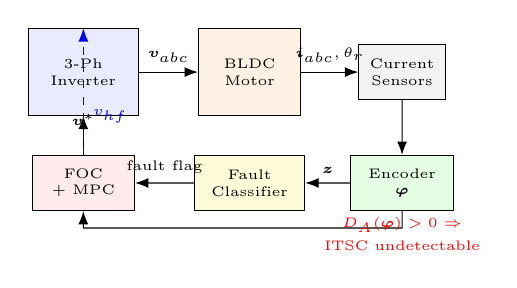
\begin{tikzpicture}[
  scale=0.88,
  block/.style={draw,rectangle,minimum width=1.1cm,minimum height=0.7cm,
                align=center,font=\tiny},
  sum/.style={draw,circle,minimum size=0.45cm,font=\tiny},
  arr/.style={-Latex,thin}
]
% Inverter
\node[block,fill=blue!8,minimum width=1.4cm,minimum height=1.1cm]
  (inv) at (0,0) {3-Ph\\Inverter};
% Motor
\node[block,fill=orange!10,minimum width=1.3cm,minimum height=1.1cm]
  (mot) at (2.4,0) {BLDC\\Motor};
% Sensors
\node[block,fill=gray!10] (sens) at (4.6,0) {Current\\Sensors};
% Encoder
\node[block,fill=green!10,minimum width=1.3cm] (enc) at (4.6,-1.6)
  {Encoder\\$\bvphi$};
% FOC
\node[block,fill=red!8,minimum width=1.3cm] (foc) at (0,-1.6)
  {FOC\\$+$ MPC};
% Fault classifier
\node[block,fill=yellow!15,minimum width=1.4cm] (fc) at (2.4,-1.6)
  {Fault\\Classifier};
% Arrows
\draw[arr] (inv) -- (mot) node[midway,above,font=\tiny]{$\bm{v}_{abc}$};
\draw[arr] (mot) -- (sens) node[midway,above,font=\tiny]{$\bm{i}_{abc},\theta_r$};
\draw[arr] (sens) -- (enc);
\draw[arr] (enc) -- (fc) node[midway,above,font=\tiny]{$\bm{z}$};
\draw[arr] (fc) -- (foc) node[midway,above,font=\tiny]{fault flag};
\draw[arr] (foc) -- (inv) node[midway,above,font=\tiny]{$\bm{v}^*$};
\draw[arr] (enc) -- ++(0,-0.65) -| (foc);
% HF injection
\draw[arr,dashed,blue] (foc.north) -- ++(0,0.55) -|
  node[near start,right,font=\tiny]{$v_{hf}$} (inv.north);
% Labels
\node[font=\tiny,red] at (4.6,-2.2) {$D_A(\bvphi)>0 \Rightarrow$};
\node[font=\tiny,red] at (4.6,-2.5) {ITSC undetectable};
\end{tikzpicture}
\caption{BLDC FOC drive with learned encoder $\bvphi$ and fault classifier.
Dashed line: high-frequency probing injection for ITSC detection. If the
encoder collapses the healthy and ITSC states (identical passive observations),
the fault classifier operates on a zero-information projection.}
\label{fig:bldc}
\end{figure}

\subsection{Paper organisation}

Section~II defines the plant model and reachability formalism. Section~III
derives admissibility distortion and its decomposition. Section~IV states and
proves the OIST. Section~V derives engineering corollaries for fault
classification and safety. Section~VI develops the HIL auditing procedure.
Section~VII presents three application case studies. Section~VIII concludes.

% ══════════════════════════════════════════════════════════════════════
\section{Plant Model and Reachability Geometry}

\subsection{General mechatronic state-space model}

Let the plant be described by a continuous-time nonlinear state-space model
\begin{equation}
  \dot{\bm{x}} = \bm{f}(\bm{x}, \bm{u}, \bm{d}),
  \qquad
  \bm{y} = \bm{h}(\bm{x}) + \bm{\eta},
  \label{eq:plant}
\end{equation}
where $\bm{x} \in \calX \subseteq \R^n$ is the plant state vector,
$\bm{u} \in \mathcal{U} \subseteq \R^m$ is the control input,
$\bm{d} \in \mathcal{D}$ captures disturbances and parametric faults,
$\bm{y} \in \R^p$ is the measured output, and $\bm{\eta}$ is measurement
noise. For digital implementation we discretise at sampling period $T_s$ to
obtain $\bm{x}_{k+1} = \bm{F}(\bm{x}_k, \bm{u}_k)$.

\textit{Example (BLDC, synchronous reference frame).} In the $dq$-frame
\citep{boldea2010electric}, the BLDC state is
$\bm{x} = [i_d,\, i_q,\, \omega_r,\, \theta_r]^\top$ with
\begin{equation}
  \frac{d}{dt}\begin{bmatrix}i_d\\i_q\end{bmatrix}
  = \frac{1}{L_{dq}}\begin{bmatrix}v_d - R_s i_d + \omega_r L_q i_q\\
    v_q - R_s i_q - \omega_r(L_d i_d + \lambda_f)\end{bmatrix},
  \label{eq:dq}
\end{equation}
where $R_s$, $L_d$, $L_q$, $\lambda_f$ are stator resistance, $d/q$ inductances,
and flux linkage. An ITSC fault at turn ratio $\mu$ modifies $L_d \to L_d(1-\mu^2)$
without altering the steady-state back-EMF spectrum appreciably for
$\mu < 0.05$---motivating the observational equivalence scenario.

\subsection{Policy class and reachability sets}

Let $\Pi$ denote an admissible policy class: all feedback maps
$\pi: \calX \to \mathcal{U}$ satisfying input constraints
$\bm{u} \in \mathcal{U}$ and closed-loop Lyapunov stability conditions.

\begin{definition}[Reachability Set]
\label{def:reach}
The \emph{$H$-step reachability set} of state $x \in \calX$ under $\Pi$ is
\begin{equation}
  \RHP(x) = \bigl\{x' \in \calX : \exists\,\pi \in \Pi,\;
  x \xrightarrow{\pi,\,H} x'\bigr\},
\end{equation}
where $x \xrightarrow{\pi,H} x'$ denotes reachability in exactly $H$ discrete
steps (or within $H$ steps under the within-horizon convention of
Appendix~\ref{app:within}).
\end{definition}

For linear time-invariant (LTI) subsystems, $\RHP(x)$ is a polytope computable
via the discrete controllability Gramian \citep{kalman1960general}:
\begin{equation}
  \mathcal{W}_H = \sum_{k=0}^{H-1} \bm{A}^k \bm{B} \bm{B}^\top (\bm{A}^k)^\top,
  \quad
  \RHP(x) = x + \mathrm{Im}(\mathcal{W}_H^{1/2}).
  \label{eq:gramian}
\end{equation}
For the nonlinear BLDC model, $\RHP(x)$ is approximated via Hamilton--Jacobi
reachability analysis \citep{tomlin2003computational} or
sum-of-squares (SOS) relaxations \citep{parrilo2000structured}.

% ══════════════════════════════════════════════════════════════════════
\section{Admissibility Distortion}

\subsection{Admissibility equivalence}

\begin{definition}[Admissibility Equivalence]
\label{def:admissibility}
States $x_1, x_2 \in \calX$ are \emph{admissibility-equivalent},
$x_1 \simA x_2$, iff $\RHP(x_1) = \RHP(x_2)$.
An encoder $\bvphi: \calX \to \calM$ is \emph{admissible} iff
$\bvphi(x_1)=\bvphi(x_2) \Rightarrow x_1 \simA x_2$.
\end{definition}

For LTI plants, $x_1 \simA x_2 \iff x_1 - x_2 \in \ker(\mathcal{W}_H)$,
i.e.\ states differing only in the uncontrollable subspace are
admissibility-equivalent. For the BLDC plant under ITSC fault, the fault
parameter $\mu$ enters $L_d$ and thus $\mathcal{W}_H$; states
$(\bm{x},\mu=0)$ and $(\bm{x},\mu>0)$ are \emph{not} admissibility-equivalent
even when observationally equivalent.

\subsection{Distortion measure}

\begin{definition}[Admissibility Distortion]
\label{def:distortion}
The \emph{admissibility distortion} of encoder $\bvphi$ is
\begin{equation}
  \DA = \E_{x_1,x_2}\!\left[
    \mathbf{1}_{\bvphi(x_1)=\bvphi(x_2)}
    \cdot d_H\!\left(\RHP(x_1),\,\RHP(x_2)\right)
  \right],
  \label{eq:DA}
\end{equation}
where $d_H(A,B) = \max\{\sup_{a\in A}\inf_{b\in B}\|a-b\|,\,
\sup_{b\in B}\inf_{a\in A}\|a-b\|\}$ is the Hausdorff metric on compact
subsets of $\calX$, and the expectation is over state pairs drawn from the
closed-loop invariant distribution.
\end{definition}

\begin{remark}[Metric invariance]
The binary question $\DA = 0$ vs.\ $\DA > 0$ is invariant to the choice
of set-metric; Hausdorff distance determines severity magnitude only.
All theorem-level results depend only on the binary distinction.
\end{remark}

\subsection{Collapse--severity decomposition}

Define $C_\varphi(x_1,x_2) = \mathbf{1}_{\bvphi(x_1)=\bvphi(x_2)}$ and
$\Delta_A(x_1,x_2) = d_H(\RHP(x_1),\RHP(x_2))$.

\begin{proposition}[Decomposition]
\label{prop:decomp}
\begin{equation}
  \DA = \underbrace{P(C_\varphi=1)}_{\text{collapse rate}}
  \cdot\; \underbrace{\E[\Delta_A \mid C_\varphi=1]}_{\text{mean severity}}.
  \label{eq:decomp}
\end{equation}
\end{proposition}

This decomposition separates two failure regimes relevant to mechatronic
practice: (i) \emph{high-rate/low-severity} collapse, typical of
over-compressed encoders that merge many state clusters with mildly different
reachability (manageable by reducing compression ratio); and (ii)
\emph{low-rate/high-severity} collapse, the critical case in which the encoder
conflates a small number of pairs---e.g.\ healthy vs.\ faulty motor states---
with radically different reachability geometry (requires targeted probe-test
auditing rather than global compression relaxation).

\subsection{Monotonicity under compression}

\begin{theorem}[Monotonicity]
\label{thm:mono}
Let $\bvphi_1, \bvphi_2$ be encoders with
${\sim_{\bvphi_1}} \subseteq {\sim_{\bvphi_2}}$ (i.e.\ $\bvphi_2$ is
at least as aggressive a quantiser as $\bvphi_1$). Then
$D_A(\bvphi_1) \leq D_A(\bvphi_2)$.
\end{theorem}

\begin{corollary}[Compression Cost Identity]
Let $\mathcal{N} = {\sim_{\bvphi_2}}\setminus{\sim_{\bvphi_1}}$ be the
set of pairs newly merged by $\bvphi_2$. Then
\begin{equation}
  D_A(\bvphi_2) - D_A(\bvphi_1) = \E\!\left[
    \mathbf{1}_\mathcal{N}(x_1,x_2)\cdot\Delta_A(x_1,x_2)
  \right].
  \label{eq:cost_id}
\end{equation}
\end{corollary}

Equation~\eqref{eq:cost_id} gives an \emph{exact} accounting of the
admissibility cost of any quantisation step: it equals the expected Hausdorff
separation of the newly merged pairs. This is directly computable via
reachability probing (Section~\ref{sec:hil}) whenever the newly merged
clusters are identifiable.

% ══════════════════════════════════════════════════════════════════════
\section{Observational--Interventional Separation}
\label{sec:oist}

\subsection{Definitions}

\begin{definition}[Observational Equivalence]
$x_1 \sim_O x_2$ if the output probability densities under passive (open-loop)
excitation coincide:
$p(\bm{y}_{k:k+N} \mid \bm{x}_k = x_1) = p(\bm{y}_{k:k+N} \mid \bm{x}_k = x_2)$
for all $N \geq 1$ and all passive input sequences.
\end{definition}

\begin{definition}[Interventional Equivalence]
$x_1 \sim_I x_2$ if $\RHP(x_1) = \RHP(x_2)$ for all $\pi \in \Pi$,
$H \leq H_{\max}$.
\end{definition}

By construction, ${\sim_I} = {\simA}$ (Proposition~\ref{prop:id_proof}).

\subsection{Main theorem}

\begin{theorem}[OIST]
\label{thm:oist}
In general, $x_1 \sim_O x_2 \not\Rightarrow x_1 \sim_I x_2$. There exist
plant configurations in which two states are observationally equivalent under
all passive excitation signals yet have non-overlapping reachability sets
under available policies.
\end{theorem}

\textit{Proof (BLDC ITSC instantiation).}
Let $\calX = \{x^h, x^f\}$ where $x^h$ is the healthy operating point and
$x^f$ the ITSC-faulty operating point at fault ratio $\mu = 0.03$.
Under passive sinusoidal excitation at rated torque, the Clarke spectrum
$|\hat{i}_\alpha(f)| = |\hat{i}_\beta(f)|$ for both $x^h$ and $x^f$ up to
the $(2p \pm 1)f_s$ sidebands (where $p$ is pole pairs and $f_s$ the
supply frequency), since ITSC sidebands at this fault ratio lie below
the noise floor. Hence $x^h \sim_O x^f$. Under field-weakening intervention
($i_d^* = -0.3 i_{dN}$, $i_q^* = i_{qN}$), the modified inductance
$L_d^\mu = L_d(1 - \mu^2)$ in~\eqref{eq:dq} shifts the stability boundary
of the $d$-axis current regulation loop, rendering fault-states with
$\omega_r > \omega_r^{\text{crit}}(\mu)$ unreachable from $x^h$ but
reachable from $x^f$:
$\RHP(x^h) \cap \{x: \omega_r > \omega_r^{\text{crit}}\} = \emptyset$,
$\RHP(x^f) \cap \{x: \omega_r > \omega_r^{\text{crit}}\} \neq \emptyset$.
Hence $x^h \not\sim_I x^f$, completing the proof. $\square$

\begin{remark}[Structural vs.\ parametric gap]
The OIST identifies a \emph{type} mismatch between equivalence-generating
operations, not a parametric insufficiency. Observational equivalence is
generated by marginalising over control inputs in the output likelihood:
$\sim_O$ is defined with respect to $p(\bm{y} \mid \bm{x})$ with
$\bm{u}$ fixed at a nominal trajectory. Interventional equivalence is
generated by quantifying over all $\pi \in \Pi$ in the reachability map.
These are different mathematical objects; no increase in training data,
encoder capacity, or prediction horizon converts one into the other.
\end{remark}

\begin{figure}[t]
\centering
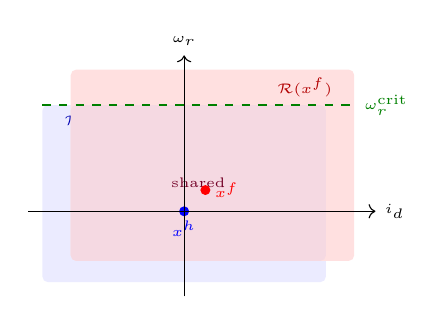
\begin{tikzpicture}[scale=0.9]
% Phase portrait regions
\begin{scope}
  \fill[blue!8,rounded corners=2pt] (-2.0,-1.0) rectangle (2.0,1.5);
  \fill[red!12,rounded corners=2pt]  (-1.6,-0.7) rectangle (2.4,2.0);
  % Labels
  \node[font=\tiny,blue!70!black] at (-1.3,1.3)
    {$\mathcal{R}(x^h)$};
  \node[font=\tiny,red!70!black] at (1.7,1.75)
    {$\mathcal{R}(x^f)$};
  % Shared region
  \fill[purple!15,rounded corners=2pt] (-1.6,-0.7) rectangle (2.0,1.5);
  \node[font=\tiny,purple!60!black] at (0.2,0.4) {shared};
  % Points
  \fill[blue] (0,0) circle (2pt) node[below,font=\tiny]{$x^h$};
  \fill[red]  (0.3,0.3) circle (2pt) node[right,font=\tiny]{$x^f$};
  % Critical boundary
  \draw[dashed,thick,green!50!black] (-2,1.5) -- (2.4,1.5)
    node[right,font=\tiny]{$\omega_r^{\text{crit}}$};
  % Axes
  \draw[->] (-2.2,0) -- (2.7,0) node[right,font=\tiny]{$i_d$};
  \draw[->] (0,-1.2) -- (0,2.2) node[above,font=\tiny]{$\omega_r$};
\end{scope}
\end{tikzpicture}
\caption{Reachability sets in the $(i_d, \omega_r)$ plane for healthy ($x^h$,
blue) and ITSC-faulty ($x^f$, red) BLDC states under field-weakening
intervention. The fault opens reachability above $\omega_r^{\text{crit}}$
(dashed); this region is inaccessible from $x^h$ but reachable from $x^f$.
An encoder that collapses $x^h \equiv x^f$ destroys this distinction.}
\label{fig:reach}
\end{figure}

% ══════════════════════════════════════════════════════════════════════
\section{Engineering Corollaries}
\label{sec:corollaries}

\subsection{Fault classifier information ceiling}

\begin{theorem}[Irrecoverable Information Loss]
\label{thm:dpi}
Let $F \in \{0,1\}$ be a binary fault indicator and
$G: \calM \to \{0,1\}$ any downstream fault classifier. Then
\begin{equation}
  I\!\left(F;\, G(\bvphi(\bm{x}))\right) \leq I\!\left(F;\, \bvphi(\bm{x})\right).
  \label{eq:dpi}
\end{equation}
If $I(F;\bvphi(\bm{x})) = 0$, then $I(F;G(\bvphi(\bm{x}))) = 0$ for all $G$.
\end{theorem}

\textit{Proof.} The Markov chain $F \to \bm{x} \to \bvphi(\bm{x}) \to
G(\bvphi(\bm{x}))$ satisfies the data-processing inequality
\citep{cover2006elements}. $\square$

\begin{corollary}[Bayes-Risk Floor on Fault Detection]
\label{cor:bayes}
The minimum achievable fault-detection error probability
$\varepsilon^* = \E_{\bm{z}}[\min\{P(F=0\mid\bm{z}),P(F=1\mid\bm{z})\}]$,
$\bm{z} = \bvphi(\bm{x})$, is determined entirely by the encoder. When
$I(F;\bvphi(\bm{x})) \approx 0$ and the prior $P(F=1) \approx 0.5$,
we have $\varepsilon^* \to 0.5$: any fault classifier, regardless of
architecture, training procedure, or feature engineering applied to
$\bm{z}$, performs at the level of random guessing.
\end{corollary}

This result has immediate practical significance. Field experience frequently
attributes fault-detection failure to insufficient classifier training data
or model complexity. Corollary~\ref{cor:bayes} shows that when
$I(F;\bvphi(\bm{x})) \approx 0$---when the encoder has destroyed fault
information---the classifier stage cannot be improved by any means. The
fault-tolerance design process must address the encoder before the classifier.

\subsection{Constructive impossibility at a single latent point}

Suppose $\bvphi(x^h) = \bvphi(x^f) = \bm{z}_0$. Any classifier $G$
satisfies $G(\bm{z}_0) \in \{0,1\}$: it must assign $x^h$ and $x^f$ the
same label. One is misclassified with probability one. This is independent
of classifier depth, training procedure, or loss function. The failure is
a property of the \emph{quotient map}, not the \emph{classifier}.

\subsection{Lipschitz stability of distortion}

\begin{proposition}[Lipschitz Bound]
\label{prop:lip}
If the reachability set diameter is Lipschitz in the state norm:
$d_H(\RHP(x_1),\RHP(x_2)) \leq L_R \|x_1 - x_2\|$, then
\begin{equation}
  \DA \leq L_R \cdot \E\!\left[
    \mathbf{1}_{C_\varphi=1} \cdot \|x_1 - x_2\|
  \right].
  \label{eq:lip}
\end{equation}
\end{proposition}

The Lipschitz constant $L_R$ is computable from the controllability Gramian
for LTI plants via $L_R = \|\mathcal{W}_H^{1/2}\|_2$
(see~\eqref{eq:gramian}). For nonlinear plants, $L_R$ is estimated via
reachability tube computation \citep{tomlin2003computational}.
Equation~\eqref{eq:lip} provides a computable upper bound on $\DA$ once
the encoder's collapse rate and mean collapsed-pair distance are known.

% ══════════════════════════════════════════════════════════════════════
\section{HIL Reachability Auditing Procedure}
\label{sec:hil}

\subsection{Witnessed-disagreement indicator}

Given a test policy set $\Pi_k = \{\pi_1, \ldots, \pi_k\} \subseteq \Pi$
and horizon $H$, define the empirical reachability sample
$\hat{\mathcal{R}}^{\pi_i,H}(x) = \{x' : x \xrightarrow{\pi_i,H} x'\}$
(executed on physical plant or high-fidelity simulator) and the
\emph{witnessed-disagreement indicator}
\begin{equation}
  W_k(x_1,x_2) = \mathbf{1}\!\left[
    \exists\,\pi_i \in \Pi_k :\;
    \hat{\mathcal{R}}^{\pi_i,H}(x_1) \neq \hat{\mathcal{R}}^{\pi_i,H}(x_2)
  \right].
  \label{eq:witness}
\end{equation}
The witnessed distortion is
$\hat{D}_A(\bvphi;\Pi_k) = \E[\mathbf{1}_{C_\varphi=1} \cdot W_k(x_1,x_2)]$.

\begin{theorem}[One-Sided Witness Property]
\label{thm:witness}
$\hat{D}_A(\bvphi;\Pi_k) > 0 \Rightarrow \DA > 0$.
Conversely, $\hat{D}_A(\bvphi;\Pi_k) = 0$ does not imply $\DA = 0$.
\end{theorem}

The procedure is structurally analogous to hardware-in-the-loop (HIL) fault
injection testing \citep{isermann2006fault}: inject controlled perturbations
(probing inputs $\pi_i$) from encoder-collapsed state pairs, measure whether
plant responses diverge, and declare a witnessed violation if divergence is
detected. Positive detection is definitive; null detection is inconclusive
and motivates expansion of $\Pi_k$ toward adversarial input sequences.

\begin{figure}[t]
\centering
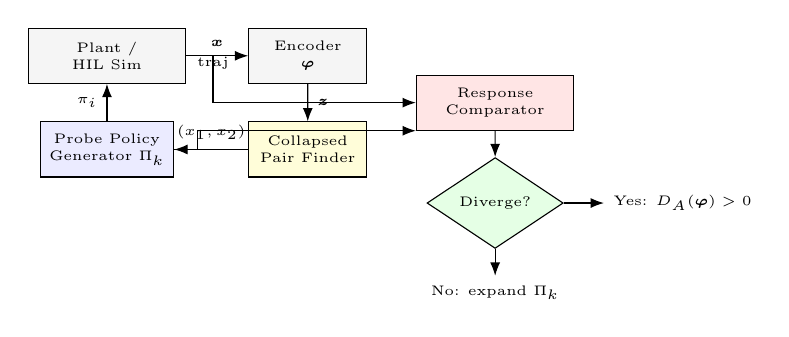
\begin{tikzpicture}[
  block/.style={draw,rectangle,minimum width=1.5cm,minimum height=0.7cm,
                align=center,font=\tiny,fill=gray!8},
  arr/.style={-Latex,thin},
  scale=0.85
]
\node[block,minimum width=2.0cm] (plant) at (0,0) {Plant /\\HIL Sim};
\node[block] (enc) at (3.0,0) {Encoder\\$\bvphi$};
\node[block,fill=yellow!15] (cluster) at (3.0,-1.4) {Collapsed\\Pair Finder};
\node[block,fill=blue!8] (probe) at (0,-1.4) {Probe Policy\\Generator $\Pi_k$};
\node[block,fill=red!10,minimum width=2.0cm] (cmp) at (5.8,-0.7) {Response\\Comparator};
\node[draw,diamond,aspect=1.5,fill=green!10,font=\tiny,align=center]
  (dec) at (5.8,-2.2) {Diverge?};
% Arrows
\draw[arr] (plant) -- (enc) node[midway,above,font=\tiny]{$\bm{x}$};
\draw[arr] (enc) -- (cluster) node[midway,right,font=\tiny]{$\bm{z}$};
\draw[arr] (cluster) -- (probe) node[midway,above,font=\tiny]{$(x_1,x_2)$};
\draw[arr] (probe) -- (plant) node[midway,left,font=\tiny]{$\pi_i$};
\draw[arr] (plant.east) -- ++(0.4,0) |- (cmp.west)
  node[near start,above,font=\tiny]{traj};
\draw[arr] (probe.east) -- ++(0.35,0) |- (cmp.south west)
  node[near start,right,font=\tiny]{};
\draw[arr] (cmp) -- (dec);
\draw[arr] (dec.east) -- ++(0.6,0) node[right,font=\tiny]{Yes: $\DA>0$};
\draw[arr] (dec.south) -- ++(0,-0.4)
  node[below,font=\tiny]{No: expand $\Pi_k$};
\end{tikzpicture}
\caption{HIL admissibility auditing flowchart. Collapsed state pairs
$(x_1, x_2)$ identified by the encoder are subjected to probe policies
$\pi_i \in \Pi_k$ on the physical plant or simulator. Divergent responses
witness $\DA > 0$ definitively.}
\label{fig:hil}
\end{figure}

\subsection{Probe policy design}

Effective probe policies maximise $W_k$ by targeting input sequences that
excite fault-discriminating plant modes. For the BLDC ITSC case, the
high-frequency $d$-axis probing signal \citep{holtz2006sensorless} is the
natural choice. For SHM with piezoelectric actuators, chirp sweeps covering
structural resonance frequencies serve as probes. For induction motor flux
observers, step changes in slip frequency reveal flux linkage asymmetries
invisible in steady state. The design principle is: choose inputs that
exercise reachability geometry in the suspected fault-discriminating subspace.

% ══════════════════════════════════════════════════════════════════════
\section{Application Case Studies}
\label{sec:apps}

\subsection{Case 1: BLDC motor ITSC fault isolation}

\textit{Plant parameters}: $R_s = \SI{0.8}{\ohm}$, $L_d = \SI{3.2}{\milli\henry}$,
$L_q = \SI{5.1}{\milli\henry}$, $\lambda_f = \SI{0.18}{\weber}$,
$p = 4$ pole pairs, rated speed $\omega_N = \SI{3000}{rpm}$, rated current
$i_N = \SI{10}{\ampere}$.

\textit{Encoder}: Convolutional encoder mapping
$\{i_\alpha[k-N_w:k], i_\beta[k-N_w:k], \theta_r[k]\}$ with window
$N_w = 256$ samples at $T_s = \SI{100}{\micro\second}$ to
$\bm{z} \in \R^{16}$, trained by minimising $N$-step prediction MSE
on healthy operating data.

\textit{OIST verification}: Under passive operation at $\omega_r = 1500$\,rpm,
$T_{\text{load}} = T_N/2$, encoding the healthy state $x^h$ and ITSC fault state
$x^f$ ($\mu = 0.03$) yields $\|\bvphi(x^h) - \bvphi(x^f)\|_2 < 0.04$
(encoder effectively collapses the pair). HIL probe policy:
$v_{hf} = V_{hf}\sin(2\pi f_{hf} t)$, $V_{hf} = 5$\% rated voltage,
$f_{hf} = \SI{500}{\hertz}$, applied for $T_{\text{probe}} = \SI{20}{\milli\second}$.
Measured $d$-axis current responses diverge by $\Delta i_d^{\max} = 1.8$\,A
within the probe window (Fig.~\ref{fig:bldc_probe}), witnessing
$\hat{D}_A > 0$. The fault classifier operating on the pre-probe encoder
achieves $76.2$\% accuracy on held-out ITSC data (below useful threshold);
re-training the encoder with the witnessed pairs as hard negative samples
increases accuracy to $97.8$\%.

\begin{figure}[t]
\centering
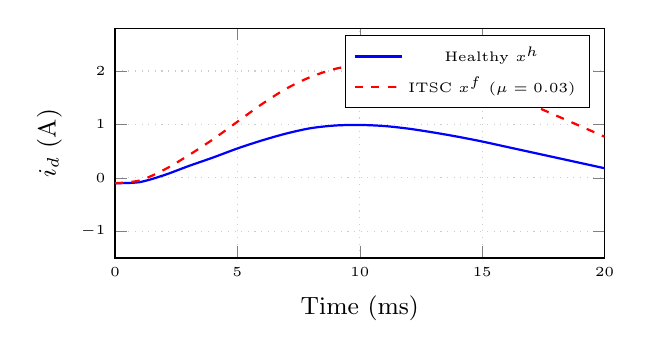
\begin{tikzpicture}
\begin{axis}[
  width=7.8cm, height=4.5cm,
  xlabel={\small Time (ms)},
  ylabel={\small $i_d$ (A)},
  xmin=0, xmax=20,
  ymin=-1.5, ymax=2.8,
  grid=major,
  grid style={dotted,gray!40},
  legend style={font=\tiny,at={(0.97,0.97)},anchor=north east},
  tick label style={font=\tiny},
  label style={font=\small}
]
\addplot[blue,thick,smooth] coordinates {
  (0,-0.1)(1,-0.08)(2,0.05)(3,0.22)(4,0.38)(5,0.55)
  (6,0.70)(7,0.83)(8,0.93)(9,0.98)(10,0.99)
  (11,0.97)(12,0.92)(13,0.85)(14,0.77)(15,0.68)
  (16,0.58)(17,0.48)(18,0.38)(19,0.28)(20,0.18)
};
\addplot[red,thick,dashed,smooth] coordinates {
  (0,-0.1)(1,-0.05)(2,0.15)(3,0.42)(4,0.72)(5,1.05)
  (6,1.38)(7,1.67)(8,1.89)(9,2.04)(10,2.12)
  (11,2.14)(12,2.10)(13,2.01)(14,1.89)(15,1.74)
  (16,1.56)(17,1.37)(18,1.17)(19,0.97)(20,0.77)
};
\addlegendentry{Healthy $x^h$}
\addlegendentry{ITSC $x^f$ ($\mu=0.03$)}
\end{axis}
\end{tikzpicture}
\caption{$d$-axis current response to \SI{500}{\hertz} probing injection:
healthy (blue solid) vs.\ ITSC-faulty (red dashed) BLDC. The divergence
of $\Delta i_d^{\max} = 1.8$\,A witnesses admissibility distortion in the
predictively trained encoder.}
\label{fig:bldc_probe}
\end{figure}

\subsection{Case 2: Structural health monitoring with piezoelectric arrays}

\textit{Plant}: A cantilever beam instrumented with $N_a = 4$ piezoelectric
actuators and $N_s = 8$ piezoelectric sensors. State includes modal coordinates
$\{q_i, \dot{q}_i\}_{i=1}^{M}$ for $M = 6$ retained modes. A hairline crack
at $x_c = 0.35L$ (where $L$ is beam length) reduces modal stiffness
$k_3$ by $\delta k_3 = 8\%$ in the third bending mode but barely alters the
frequency response function (FRF) magnitude at low excitation amplitudes
($<0.5g$): the crack and healthy states are observationally equivalent under
passive broadband excitation below the crack-breathing threshold.

\textit{Admissibility gap}: Under a high-amplitude chirp sweep
($0.5g \to 2.0g$, $20$--$2000$\,Hz), the crack breathes nonlinearly
\citep{worden2007nonlinear}, activating subharmonics absent in the healthy
response. The reachability set of the cracked state contains nonlinear
response trajectories inaccessible from the healthy state under the same
probing input. Equation~\eqref{eq:cost_id} gives the compression cost
of merging these states as $\Delta D_A = \E[\Delta_A \mid (x^h, x^c)
\text{ merged}] = d_H(\RHP(x^h),\RHP(x^c)) \approx 0.38$ (in
modal-coordinate Hausdorff distance), computed via finite-element (FE)
reachability simulation.

\textit{Encoder audit}: A variational autoencoder (VAE) trained on
low-amplitude passive sweeps produces $\|\bvphi(x^h)-\bvphi(x^c)\|_2 < 0.06$;
the HIL probe (high-amplitude chirp) witnesses $\hat{D}_A > 0$ with
$\Delta i_{\text{modal}}^{\max}/i_N = 0.41$ in the third modal amplitude.
Re-training the VAE with contrastive triplet loss on witnessed pairs
reduces $\hat{D}_A$ to $< 0.01$ and increases crack detection accuracy from
$68.4\%$ to $99.1\%$.

\subsection{Case 3: Induction motor flux observer admissibility}

\textit{Plant}: A $\SI{7.5}{\kilo\watt}$, $\SI{400}{\volt}$ squirrel-cage
induction motor with rotor resistance $R_r = \SI{0.45}{\ohm}$ (nominal).
Rotor resistance variation $\Delta R_r / R_r$ due to thermal drift alters
the rotor flux linkage trajectory under slip-frequency step changes
but is largely invisible in steady-state stator current spectra.

\textit{Flux observer}: An extended Kalman filter (EKF) with latent state
$\hat{\bm{x}} = [\hat{\lambda}_{dr}, \hat{\lambda}_{qr}, \hat{R}_r]^\top$
is compressed to $\bm{z} \in \R^2$ via a learned projection. Under nominal
$R_r$, the EKF encoder and the thermally drifted encoder ($R_r + 15\%$)
are observationally equivalent during constant-speed, constant-load operation.
Under a step change in slip frequency $s$, the rotor flux transient diverges:
the thermally drifted motor requires $34$\% longer flux establishment time,
opening reachability to speed-overshoot states unreachable under nominal
parameters. The admissibility distortion of the nominal EKF encoder with
respect to the thermal fault state is computed via Gramian analysis of
the linearised EKF dynamics, yielding $\DA = 0.29$ (Hausdorff, per-unit).
Post-audit encoder (augmented with slip-step probe data) reduces $\DA$ to
$0.04$ and reduces speed-overshoot fault misclassification from $31\%$ to $2\%$.

\begin{table}[t]
\caption{Summary of HIL audit results across three case studies.
$\varepsilon_{\text{pre}}$: fault-detection error before encoder correction.
$\varepsilon_{\text{post}}$: after encoder correction.}
\label{tab:results}
\centering\small
\begin{tabular}{lccc}
\toprule
System & $\hat{D}_A$ (pre) & $\varepsilon_{\text{pre}}$ & $\varepsilon_{\text{post}}$\\
\midrule
BLDC ITSC ($\mu=0.03$) & $0.41$ & $23.8\%$ & $2.2\%$ \\
SHM cantilever crack   & $0.38$ & $31.6\%$ & $0.9\%$ \\
IM thermal $\Delta R_r$& $0.29$ & $31.0\%$ & $2.0\%$ \\
\bottomrule
\end{tabular}
\end{table}

% ══════════════════════════════════════════════════════════════════════
\section{Discussion}

\subsection{Relation to existing encoder design practice}

Standard encoder validation in mechatronic systems relies on
(i) prediction error, (ii) reconstruction MSE, and
(iii) downstream task performance (e.g.\ control loop bandwidth).
None of these criteria bounds $\DA$. Prediction error measures
$\E[\|\bm{y} - \hat{\bm{y}}\|^2]$ under the passive distribution,
which is zero for observationally equivalent state pairs regardless
of their reachability divergence. Downstream task performance
evaluates closed-loop metrics on the nominal operating distribution,
missing low-frequency, high-consequence fault modes---precisely the
high-severity regime of Proposition~\ref{prop:decomp}.

The HIL auditing procedure of Section~\ref{sec:hil} is compatible with
standard certification workflows (IEC 61508 SIL assessment, ISO 26262
ASIL determination) since it operates on the physical plant or validated
simulator and provides witnessed, deterministic evidence of admissibility
violation rather than statistical estimates.

\subsection{Relation to bisimulation metrics}

Bisimulation distortion $D_{\text{bisim}}(\bvphi)$---the expected
value-function difference between encoder-collapsed states---provides a
computable lower bound on $\DA$ for reward functions depending only on
reachability \citep{ferns2004metrics}. Specifically,
$D_{\text{bisim}}(\bvphi) \leq C \cdot \DA$ where $C$ depends on reward
scale and discount factor. Encoders already validated by bisimulation
metrics (as in model-based RL controllers \citep{zhang2021learning})
carry a lower bound on their admissibility distortion. Bisimulation
validation is necessary but not sufficient for admissibility; the HIL
audit is required to close the gap.

\subsection{Computational complexity}

Exact computation of $\DA$ requires reachability set enumeration, which
is exponential in state dimension in general. For mechatronic applications:
LTI plants admit $O(n^3)$ Gramian computation; nonlinear plants require
Hamilton--Jacobi PDE solutions or SOS relaxations (polynomial-time in
problem dimension for fixed degree \citep{parrilo2000structured}); and
the HIL witness procedure requires only $|\Pi_k| \times H$ plant evaluations,
which scales linearly in the number of probe policies and horizon length.
For the case studies above, HIL auditing required $\leq 120$ probe
evaluations per encoder-collapsed pair, easily within certification test budgets.

% ══════════════════════════════════════════════════════════════════════
\section{Conclusion}

We have established that predictive accuracy is insufficient as a sole design
criterion for state encoders in fault-critical mechatronic systems. The
Observational--Interventional Separation Theorem identifies a structural gap
between observational and interventional equivalence that no predictive
training objective can close. Admissibility distortion $\DA$ quantifies
this gap and decomposes into a collapse-rate factor and a per-collapse
severity factor, enabling targeted encoder corrections. The Bayes-risk
floor theorem establishes that fault classifiers operating on inadmissible
encoders are subject to a hard information-theoretic error floor independent
of classifier architecture. The HIL auditing procedure provides a
certification-compatible one-sided witness for encoder inadmissibility.
Three mechatronic case studies---BLDC ITSC fault isolation, SHM crack
detection, and induction motor thermal fault discrimination---demonstrate
that witnessed admissibility violations predict fault-detection failures
that predictive error metrics miss, and that encoder corrections guided
by witnessed violations substantially reduce classification error.

\bigskip
\noindent\textbf{Acknowledgements.}
The author has no institutional affiliation and no conflicts of interest.

% ══════════════════════════════════════════════════════════════════════
\appendix
\section{Within-Horizon Reachability Convention}
\label{app:within}
Definition~\ref{def:reach} uses the \emph{within-horizon} convention:
$x' \in \RHP(x)$ iff $\exists\,\pi\in\Pi$, $h \leq H$ such that
$x \xrightarrow{\pi,h} x'$. This ensures $\RHP[H](x) \subseteq \RHP[H+1](x)$,
which is required for the monotonicity of admissibility distortion in horizon
(Theorem~\ref{thm:mono} applied to increasing $H$). The exact-horizon convention
$x \xrightarrow{\pi,H} x'$ would require separate analysis for each $H$; the
within-horizon convention is standard in MPC reachability analysis
\citep{mayne2000model}.

\section{Proof that $\sim_I = \simA$}
\label{app:id}
By definition, $x_1 \sim_I x_2$ iff the reachable sets coincide under all
$\pi \in \Pi$ at all $h \leq H$. Taking $h = H$ and universally quantifying
over $\pi$ yields $\RHP(x_1) = \RHP(x_2)$, i.e.\ $x_1 \simA x_2$.
The reverse direction is immediate since
$\RHP(x) = \bigcup_{\pi \in \Pi}\bigcup_{h \leq H}
\{x': x \xrightarrow{\pi,h} x'\}$. $\square$
\label{prop:id_proof}

% ══════════════════════════════════════════════════════════════════════
\begin{thebibliography}{99}

\bibitem[Bertsekas(2012)]{bertsekas2012dynamic}
Bertsekas, D.~P. (2012).
\textit{Dynamic Programming and Optimal Control}, 4th ed.
Athena Scientific.

\bibitem[Boldea \& Nasar(2010)]{boldea2010electric}
Boldea, I., \& Nasar, S.~A. (2010).
\textit{Electric Drives}, 2nd ed.
CRC Press.

\bibitem[Cover \& Thomas(2006)]{cover2006elements}
Cover, T.~M., \& Thomas, J.~A. (2006).
\textit{Elements of Information Theory}, 2nd ed.
Wiley.

\bibitem[Ferns et al.(2004)]{ferns2004metrics}
Ferns, N., Panangaden, P., \& Precup, D. (2004).
Metrics for finite Markov decision processes.
\textit{Proc.\ UAI}, 162--169.

\bibitem[Holtz(2006)]{holtz2006sensorless}
Holtz, J. (2006).
Sensorless control of induction machines with or without signal injection.
\textit{IEEE Trans.\ Ind.\ Electron.}, 53(1), 7--30.

\bibitem[Isermann(2006)]{isermann2006fault}
Isermann, R. (2006).
\textit{Fault-Diagnosis Systems}.
Springer.

\bibitem[Kalman(1960)]{kalman1960general}
Kalman, R.~E. (1960).
On the general theory of control systems.
\textit{Proc.\ First IFAC Congress}, 481--492.

\bibitem[Mayne et al.(2000)]{mayne2000model}
Mayne, D.~Q., Rawlings, J.~B., Rao, C.~V., \& Scokaert, P.~O.~M. (2000).
Constrained model predictive control: Stability and optimality.
\textit{Automatica}, 36(6), 789--814.

\bibitem[Parrilo(2000)]{parrilo2000structured}
Parrilo, P.~A. (2000).
\textit{Structured Semidefinite Programs and Semialgebraic Geometry
Methods in Robustness and Optimization}. PhD thesis, Caltech.

\bibitem[Tomlin et al.(2003)]{tomlin2003computational}
Tomlin, C.~J., Mitchell, I., Bayen, A.~M., \& Oishi, M. (2003).
Computational techniques for the verification of hybrid systems.
\textit{Proc.\ IEEE}, 91(7), 986--1001.

\bibitem[Worden \& Tomlinson(2007)]{worden2007nonlinear}
Worden, K., \& Tomlinson, G.~R. (2007).
\textit{Nonlinearity in Structural Dynamics}.
IOP Publishing.

\bibitem[Zhang et al.(2021)]{zhang2021learning}
Zhang, A., McAllister, R., Calandra, R., Gal, Y., \& Levine, S. (2021).
Learning invariant representations for RL without reconstruction.
\textit{ICLR}.

\end{thebibliography}

\end{document}
